\documentclass[a4paper]{jacow}

\usepackage{url}
\usepackage{mathtools}
\usepackage{subcaption}
\newcommand{\barn}{\bar n}

\begin{document}
	\title{A FEASIBILITY STUDY INTO THE QUASI-FROZEN SPIN REGIME OF OPERATION OF THE NICA STORAGE RING}
	\author{A. Aksentev\textsuperscript{1}\thanks{a.aksentyev@inr.ru}, 	A. Melnikov, Y. Senichev, Institute for Nuclear Research\\ of the Russian Academy of Sciences, Moscow, Russia \\
		S. Kolokolchikov, International Union of Pure and Applied Physics, Geneve, Switzerland \\
		V. Ladygin, E M Syresin and A. Butenko, Joint Institute for Nuclear Research (JINR), Dubna, Russia\\
		\textsuperscript{1}also at National Research Nuclear University ``MEPhI,'' Moscow, Russia
	}
	\maketitle

	\begin{abstract}
		This study is motivated by the search for the electric dipole moment (EDM) of elementary particles. The most promising idea in that regard is the ``Frozen Spin'' concept first proposed by the BNL. This concept, however, requires the building of a brand-new facility devoted to the EDM-search. NICA is not such a facility, hence the need for a modification compatible with the existing optics; one that wouldn’t disrupt the ring’s capability for parallel experiments. Such a modification is the ``Quasi-Frozen Spin'' idea, realized by adding transport channels, bypassing the ring’s straight sections. Wien-filters are placed in these channels in order to compensate spin-rotations caused by the ring’s arc dipoles, thus making its net spin-transfer matrix unitary. Even though, during its movement along the beam line, the beam’s polarization vector deviates from alignment with the momentum vector, this motion is regular and fits within one beam revolution, allowing for the buildup of the EDM-signal. The present study shows that the ``Quasi-Frozen Spin''-specific optics is consistent with the existing NICA lattice and that the modified structure is capable of maintaining a requisite spin-coherence time.
	\end{abstract}

\section{THE FROZEN AND QUASI-FROZEN LATTICES}
\subsection{Frozen spin and its lattice requirements}
The motivation for this study is the search for the electric dipole moments (EDMs) of elementary particles. In an accelerator ring environment the most promising measurement idea, which grounds the ``Frozen Spin'' accelerator design concept, was first proposed by a collaboration from the Brookhaven National Laboratory (Brookhaven, USA).~\cite{AGS4deuterons} The idea consists in ``freezing'' the beam's polarization vector's orientation with respect to the momentum vector, which opens the possibility of a steady build-up of the vertical polarization vector component indicating the presence of the EDM.

The original idea, however, cannot be implemented in just any storage ring. The ``freezing'' meant here implies that the ring-plane projections of the polarization and momentum vectors are invariably aligned at any point along the beamline. Since the momentum vector rotates in the accelerator arcs by means of the guiding magnetic field, the polarization vector must also turn there simultaneously and by the same angle. The spin-rotation angle is related to the momentum one via the spin tune $\nu$ as in $\Phi_{spin} = \nu\cdot\Phi_{mom}$, and the spin-tune expressions, according to the T-BMT equation (written in the center-of-mass coordinate system), are~\cite{ICAP15:Lattices}
\begin{equation}\label{eq:spin-tune}
	\begin{cases}
		\nu^{B} &= \gamma\cdot G,\\
		\nu^{E} &= \beta^2\gamma\cdot\left(\frac{1}{\gamma^2-1} - G\right).
	\end{cases}
\end{equation}

The ``frozen spin'' condition, by requiring the spin-rotation relative to the momentum rotation to be zero, implies that the B-field spin-rotation must be compensated by an E-field one; hence the storage ring arc-elements realizing this condition are no usual dipoles, but rather cylindrical Wien-filters (E+B elements), as in Fig.~\ref{fig:FS-lattice}. The building of a brand-new facility dedicated to the experimental program is thus required.

\begin{figure}[h]
	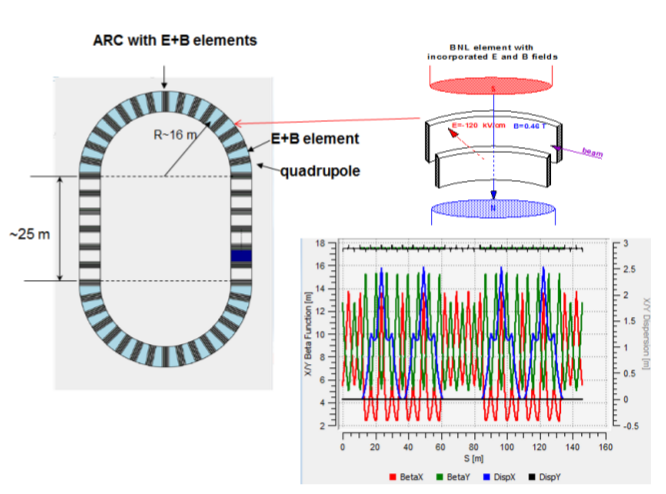
\includegraphics[width=\linewidth]{img/MOPA071_f1}
	\caption{A possible lattice with cylindrical Wien-filters for the realization of the frozen spin condition.\label{fig:FS-lattice}}
\end{figure}

Apart from this inconvenience, there are further motives to look for an alternative. One might ask oneself, whence came the frozen spin (FS) condition in the first place? As mentioned above, it is grounded in the idea of measuring the rate of the beam polarization vector's vertical component buildup. This buildup is the linear part of the general spin-precession described by the T-BMT equation. The immediate observable being the angle-of-rotation of the polarization vector, i.e. the phase $\Theta$ of the $P_V (t) = P_0\sin \Theta(t) \approx P_0(\omega t + \Theta_0)$ process, the method intended here is of the so-called ``phase'' or ``space domain'' variety. The FS-condition for such methods is the condition-of-possibility, both with respect to the linearization of the observable $P_V(t)$ and also with respect to systematic errors (the so-called ``geometrical phase'' error due to the non-commutativity of spin-rotations).

\subsection{Quasi-frozen spin and the NICA collider}
But what if, instead of using the integral value $\Theta(t)$, one uses the spin precession frequency $\omega$ as the experimental observable? Methods of this variety fall into the ``frequency domain'' category, and do not require a strict observance of the FS-condition. Neither are they sensitive to the geometrical phase error. As a consequence, the E- and B-field actions on the beam's polarization vector can be spatially separated, thus resulting in the so-called ``quasi-frozen spin'' (QFS) regime of operation. In terms of the spin-transfer matrix, the FS and QFS lattices are indistinct (hence the name, ``quasi-frozen''); but now, one might leave the existing accelerator's arcs untouched, only adapting the straight sections to the task.

Now turning to the NICA collider (JINR, Dubna, Russia), originally designed for heavy-ion experiments, if it is to be used for EDM-measurement it needs first to be turned into a storage ring capable of maintaning the beam's spin-coherence time (SCT) at the level of 1,000~seconds. This could be realized by inserting bypass channels to circumvent the existing straight sections (see Fig.~\ref{fig:NICA+bypass}). The bypass optics design considerations with respect to orbital dynamics are presented in~\cite{Kolokolchikov:Bypass}. The QFS state is brought about by E+B elements (Wien filters) placed in the ``ByPass'' straight sections (Fig.~\ref{fig:NICA+bypass}).

\begin{figure}[h]
	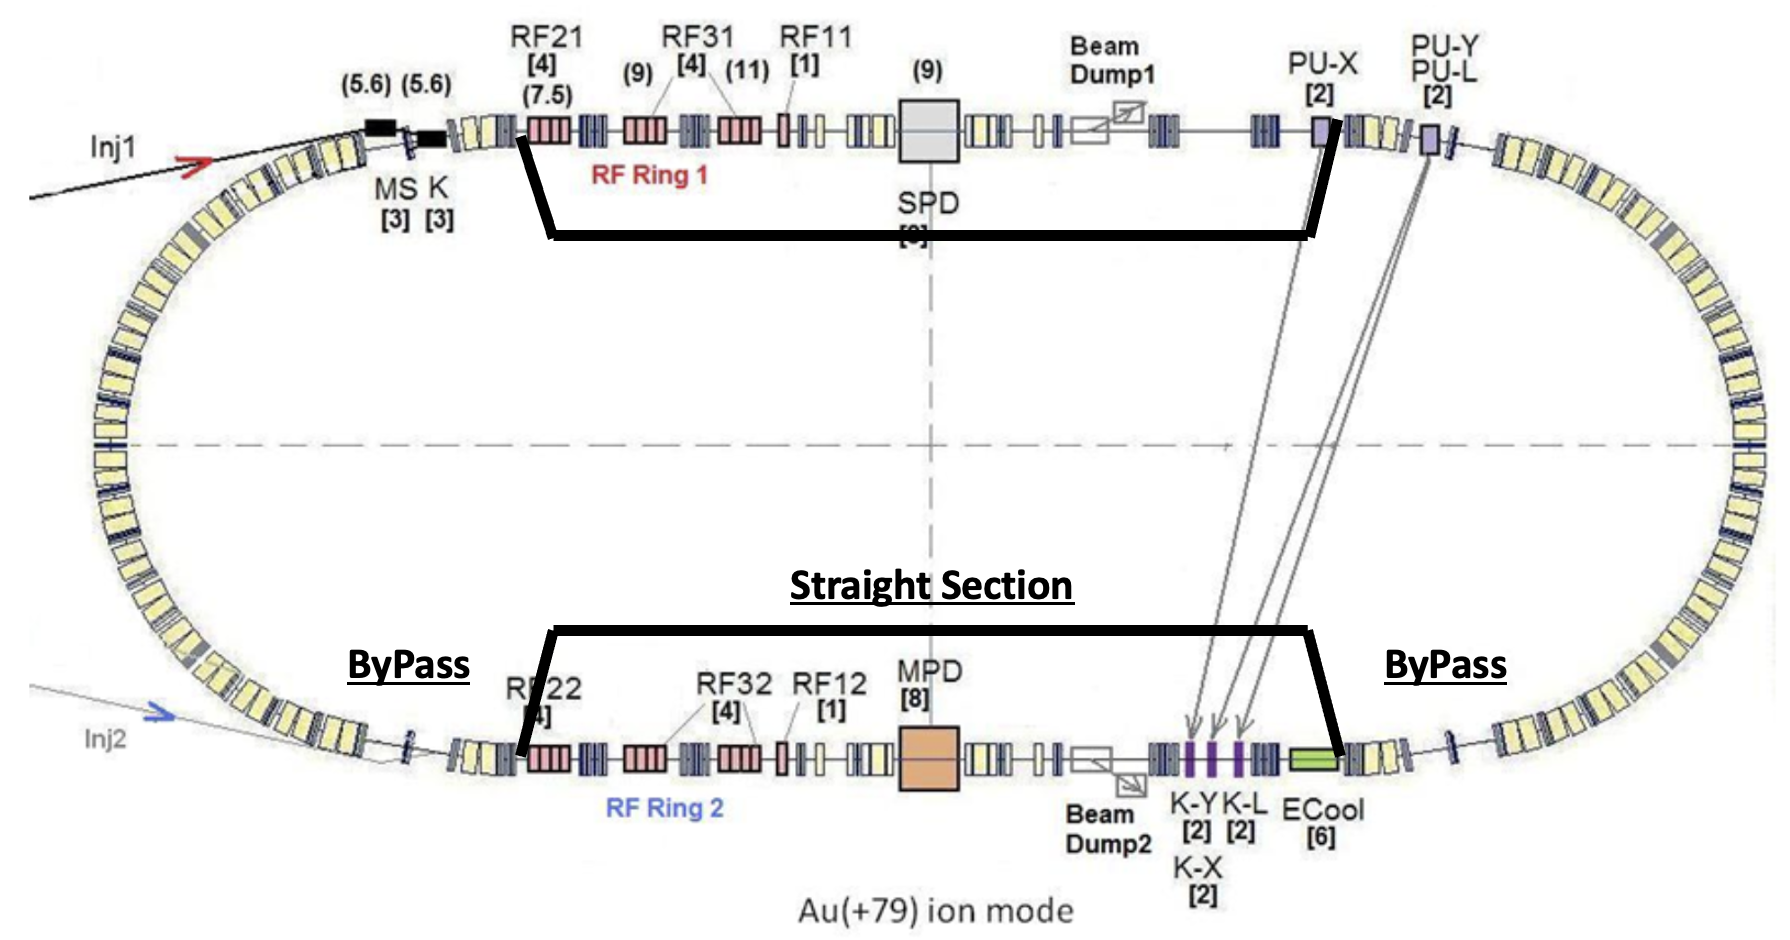
\includegraphics[width=\linewidth]{img/MOPA071_f2}
	\caption{NICA with bypass transport channels to realize the quasi-frozen spin mode.\label{fig:NICA+bypass}}
\end{figure}

\section{PREFERENCE OF THE LATTICE DESIGN CONCEPT WITH RESPECT TO THE EDM MEASUREMENT}

It is not uninteresting to summarize some of the general motivations in favor of one or the other lattice design concept.

The two parameters by which we categorize the lattices in the following are : (1) the methodological principle of EDM-measurement and (2) constuctional practicability.

With respect to the former, FS is the lattice of choice when one wishes to implement a ``space domain'' method of EDM-measurement, that is to utilize the polarization deviation angle from the ring plane as measure. Since the non-commutativity of spin-rotations prevents asynchronous compensation of a B-field rotation moved by the magnetic dipole moment (MDM) in the arc by a corresponding E-field rotation in the straight section, one wants a lattice in which the MDM spin rotation is neutralized, that is the MDM has zero instantaneous power. The FS-lattice is such a design concept. The QFS lattice, in which the compensation is by design asynchronous, would not suit such a category of methods.

On the other hand, the FS-lattice is also suitable with respect to the ``frequency domain'' method variety. So, the FS-lattice is more versatile in terms of method, while the QFS is more restricted in this regard.

But with respect to constructional viability, the situation is reverse. The asynchronicity characteristic of the QFS-design makes it implementable in any existing storage ring. One need not construct a single-purpose, dedicated ring. If one considers the further restrictions on the ring imposed by the ``space domain'' concept (such as the requirement to reduce all MDM contribution to spin-precession to below the EDM one~\cite{Senichev-FDM}), it becomes even less attractive.

To summarize, ``space domain'' methodology favors the FS design, while constructional considerations the QFS one. The latter also make the ``frequency domain'' methodology preferable, as well as, we argue in~\cite{Senichev-FDM}, the physical unviability essentially determining the ``space domain'' concept.

\section{INVESTIGATED QUESTIONS}

We are concerned with modifying an existing lattice in order to make it suitable to making EDM-measurements. This implies that the lattice must be capable of operating in the quasi-frozen spin regime, and that the beam's spin-coherence time is sufficiently long. It is proposed that the first could be relized by placing Wien filters in the lattice straight sections; the standard technology for realizing the second condition is the use of several sextupole families to correct for betatron and spin chromaticities. Both of these propositions were investigated numerically, using the COSY Infinity code.~\cite{COSY-Infinity}

In the standard formalism, the lattice's spin-transfer matrix is an SO(3) rotation matrix parameterized by the normalized spin precession frequency, spin tune, $\nu$, and the invariant spin axis $\barn$ : $T(\nu, \barn)$. If either the Q/FS holds, $T$ equals the identity matrix, and the spin tune $\nu=0$. In the proposed modification this is done by adjusting the EB element's E-field (the B-field follows to preserve the closed orbit). Numerical simulation shows that it is indeed possible to zero the beam's reference particle's spin tune $\nu_0$, as evidenced by Fig.~\ref{fig:nu-vs-EBE}.

\begin{figure}[h]
	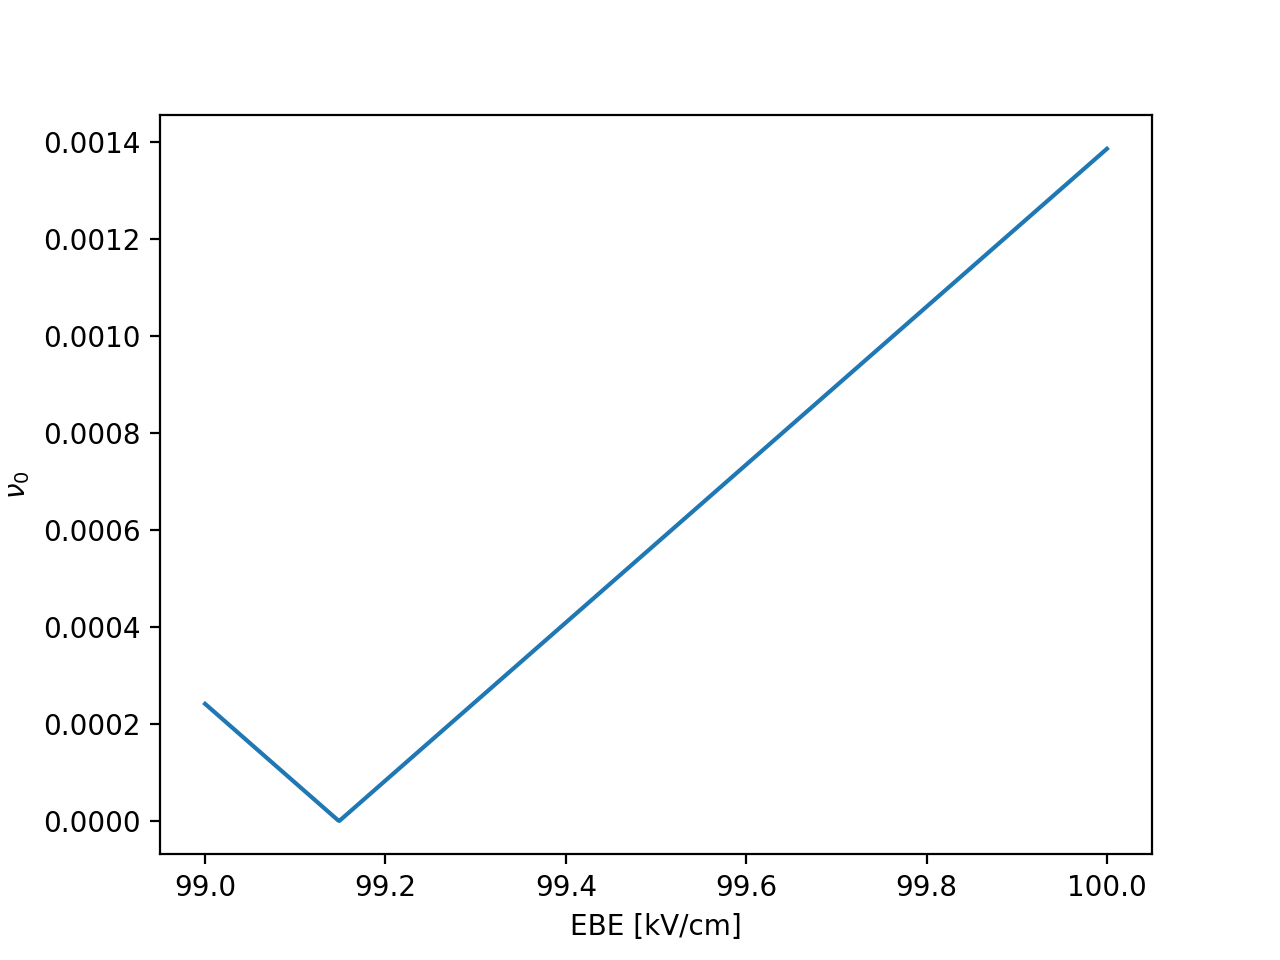
\includegraphics[width=\linewidth]{img/MOPA071_f3}
	\caption{Reference particle spin tune $\nu_0$ dependence on the EB-element's E-field.\label{fig:nu-vs-EBE}}
\end{figure}

Spin chromaticity is the dependence of a particle's spin tune on its orbit length. It results in the beam particles' spin-vectors dispersing about the invariant spin axis $\barn$, the process called ``spin decoherence.'' This process is unimportant for experiments dealing with the non-zero expectation value beam polarization; however, for EDM experiments the part of polarization orthogonal to $\barn$ is of interest, one whose expectation value is zero -- hence the significance of the term ``spin coherence time.''

The question of whether the beam's spin chromaticity can be reduced by means of sextupole families to a level providing an adequately long spin coherence time has also been answered in the positive (for an illustration please see Fig.~\ref{fig:spin-on-sext}). One should note, however, that classically, three sextupole families should be used, located respectively in the maximums of the $\beta_x$, $\beta_y$, and $D$ functions~\cite{Decoherence-main};  the lattice design does not allow for an effective separation between all three Twiss functions, hence only two families could be used in the simulation. Another point of concern is that in this setup both the betatron chromaticity and the spin chromaticity could not be simultaneously reduced.~\cite{Kolokolchikov:Coherence}

\begin{figure}[h]
	\begin{subfigure}{\linewidth}
		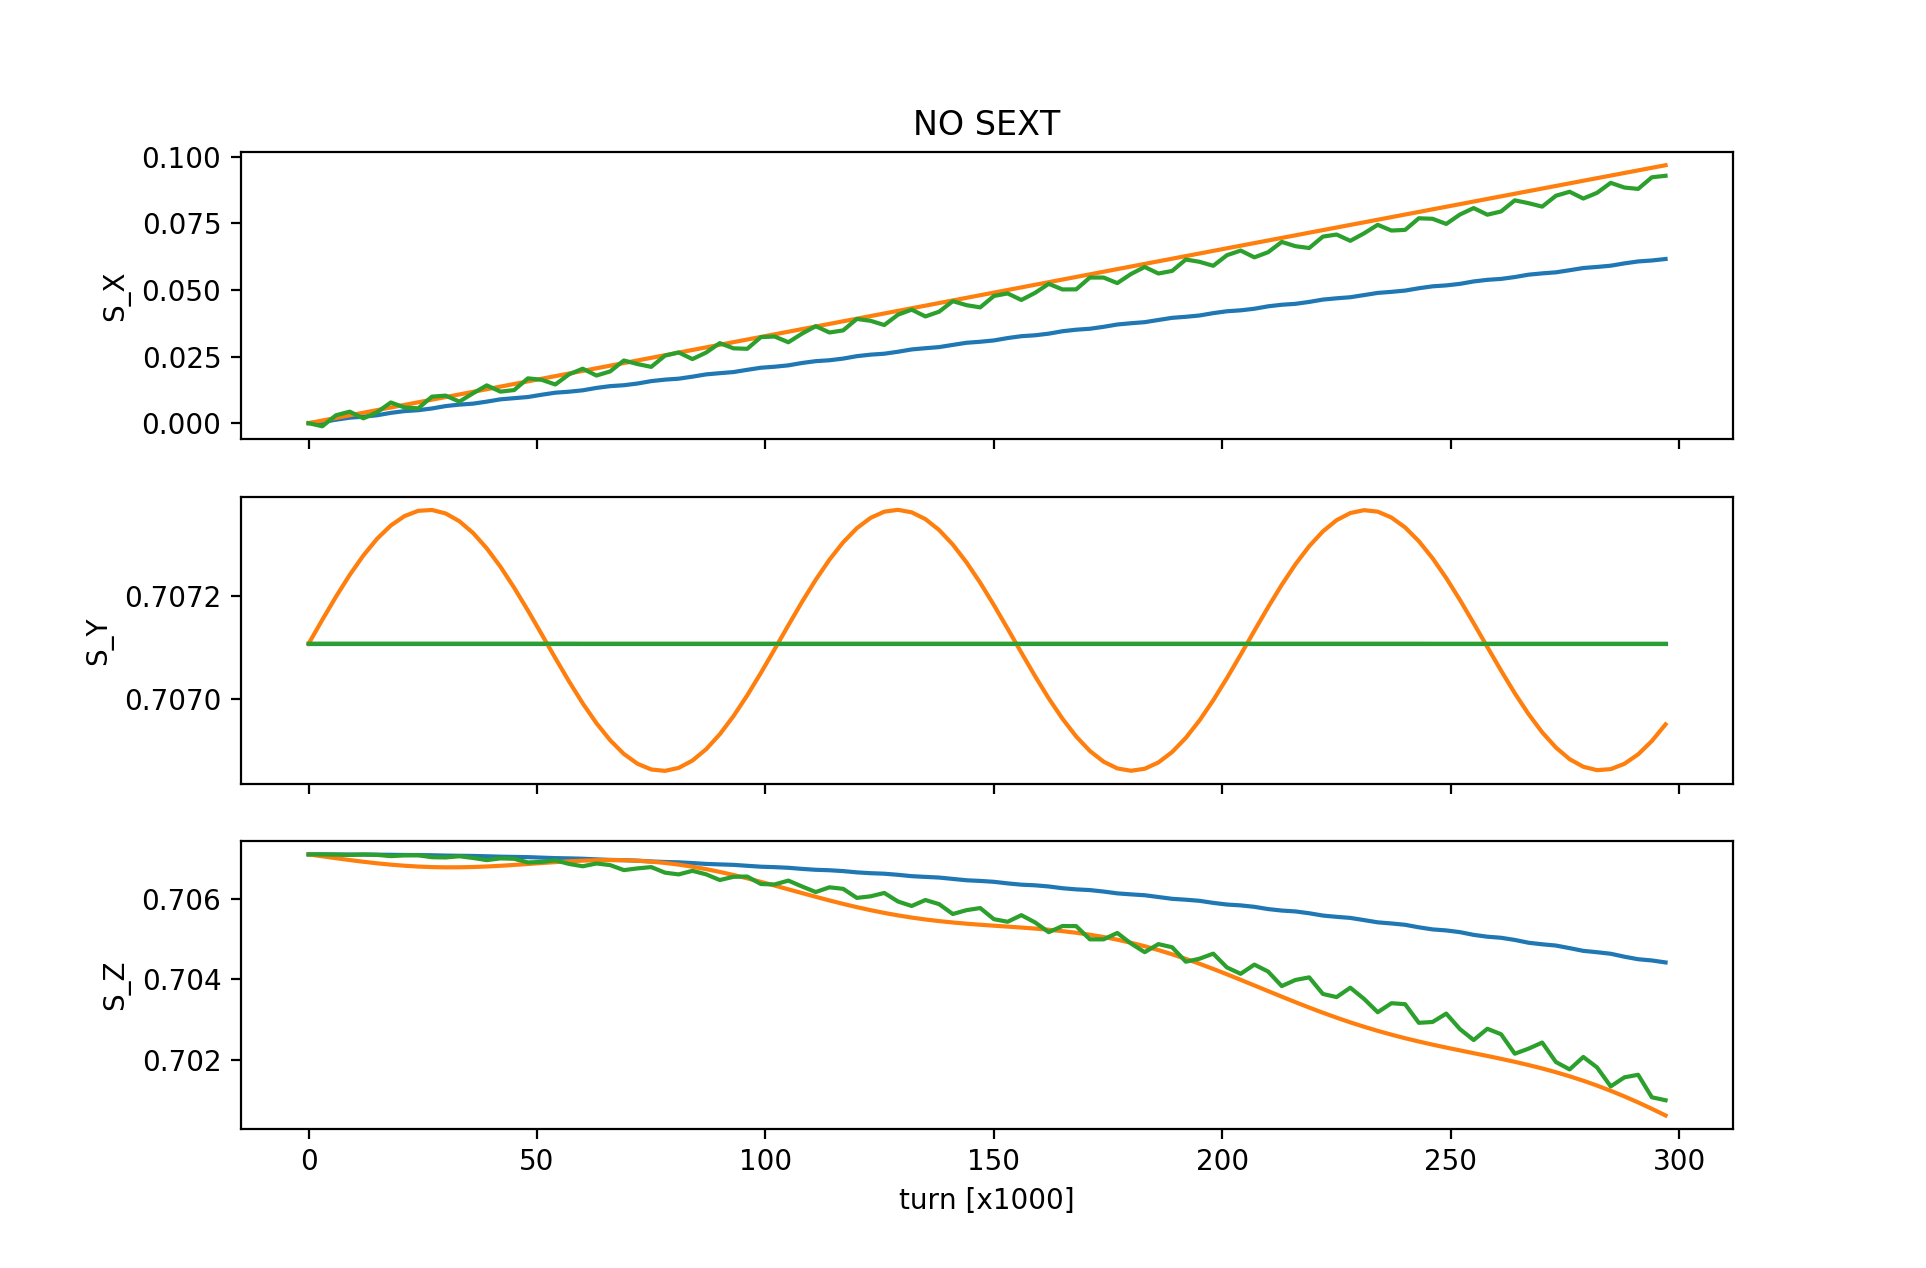
\includegraphics[width=\linewidth]{img/MOPA071_f4a}
		\caption{Sextupoles off, dispersion present.}
	\end{subfigure}
	\begin{subfigure}{\linewidth}
		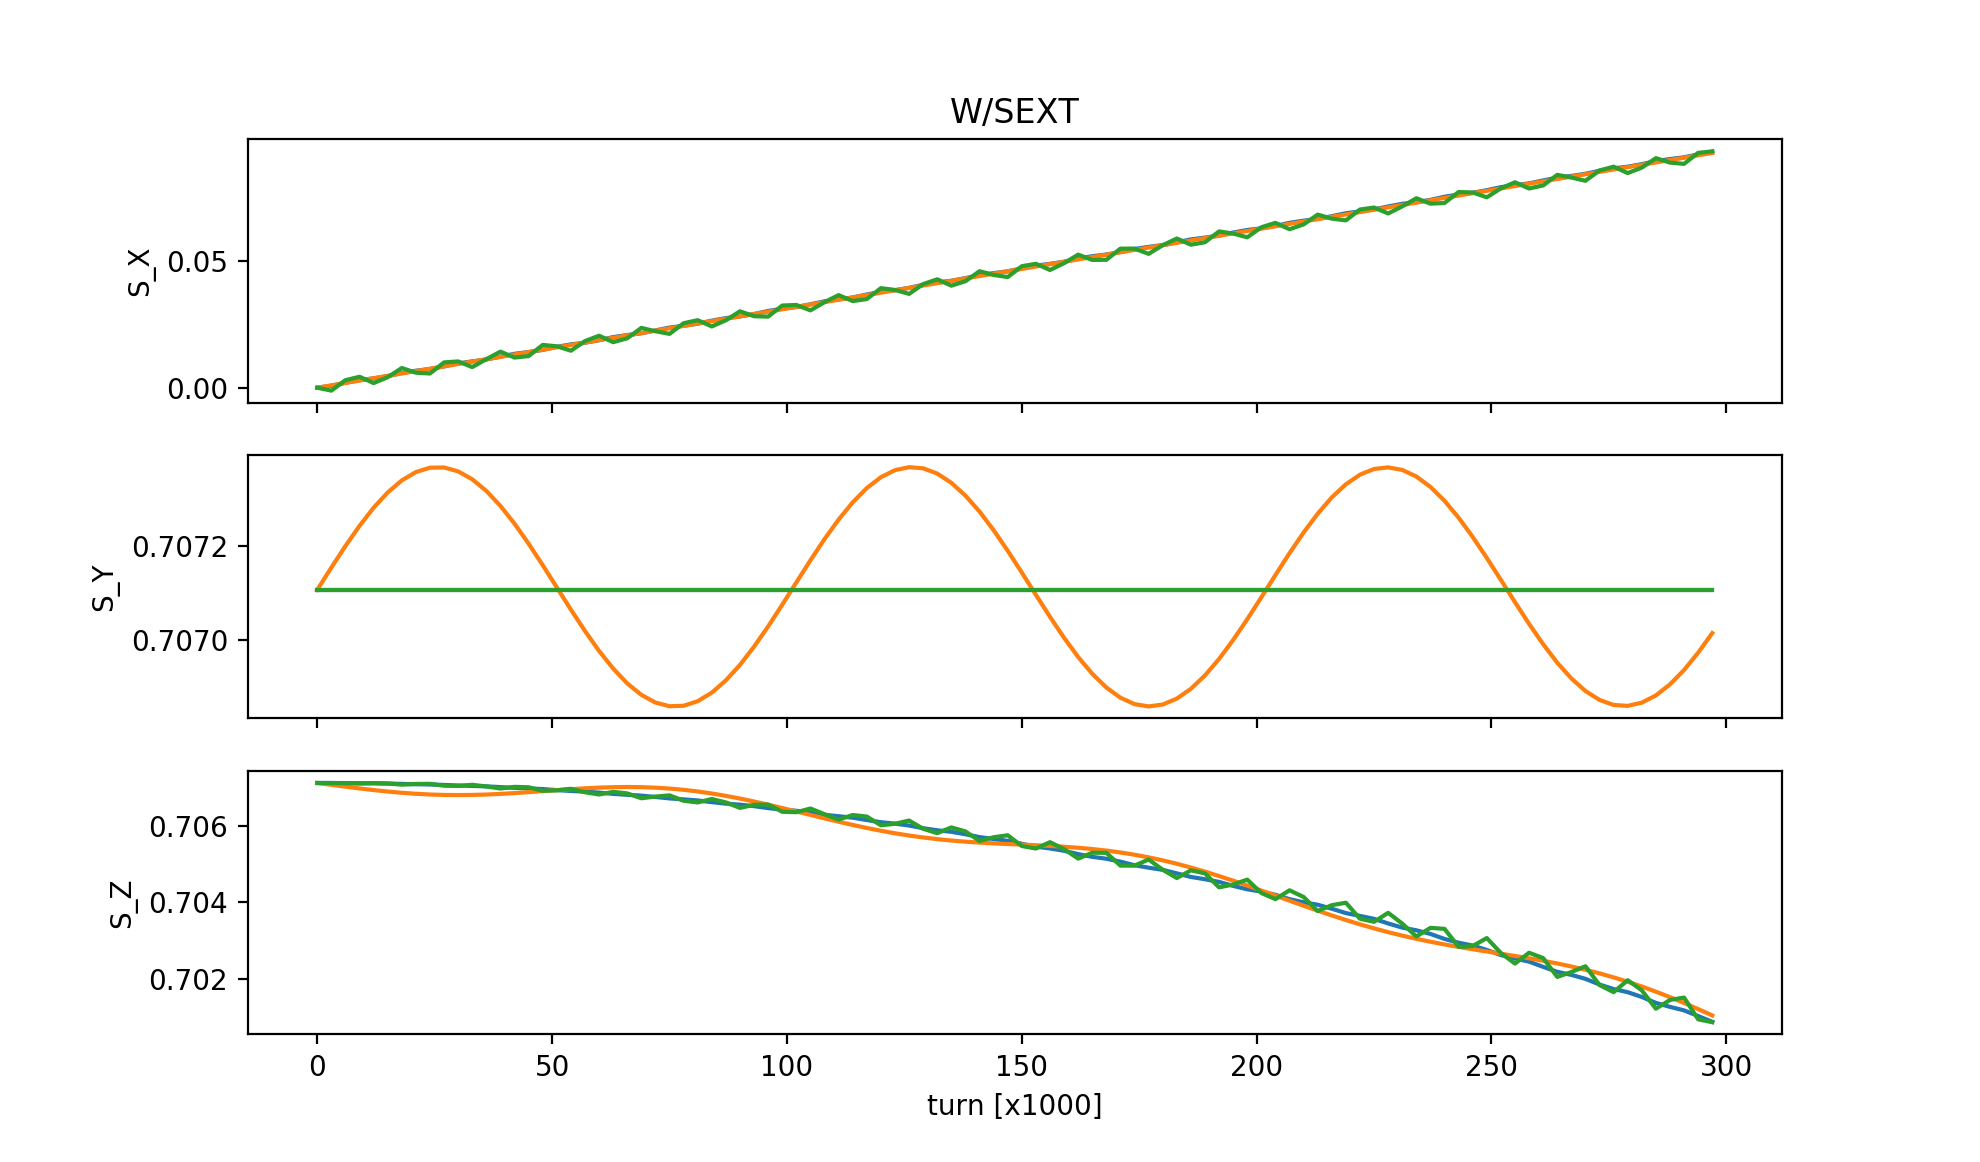
\includegraphics[width=\linewidth]{img/MOPA071_f4b}
		\caption{Sextupoles on, dispersion reduced.}
	\end{subfigure}
	\caption{Spin vector components as functions of beam revolution number in the absence and presence of sextupole families.\label{fig:spin-on-sext}}
\end{figure}


\section{CONCLUSION}
We have considered the possibility of adapting the existing NICA lattice to the purpose of EDM measurement. Two basic questions that needed to be answered in this regard are whether the quasi-frozen spin regime could be implemented and whether the modified lattice could maintain a requisite spin-coherence time.

It has been shown that the quasi-frozen spin optics are indeed consistent with the NICA arcs~\cite{Kolokolchikov:Bypass}. With regard to the second question the situation is more complex. The present design does not allow for an effective separation of chromaticity-correcting sextupoles into three families due to the reularity of the dispersion function. This results in the impossibility of simultaneously reducing both the spin and betatron chromaticities. Possible solutions to this problem have been proposed~\cite{Kolokolchikov:Coherence}. In any case, it warrants a further research.


%\section*{ACKNOWLEDGMENTS}
%We appreciate the support of this study by the Russian Science Foundation grant 22-42-04419.

%\section*{References}
\begin{thebibliography}{9}
	\bibitem{AGS4deuterons}
		D.~Anastassopoulos \textit{et al.}, (srEDM Collaboration),``Search for a permanent electric dipole moment of the deuteron nucleus at the $10^{-29}~e\cdot$ cm level,'' proposal as submitted to the BNL PAC, April 2008. \url{https://inspirehep.net/files/9ed0c86eedb4efd3213fc63fb8d7868f}
	\bibitem{ICAP15:Lattices}
		Yu.~Senichev \textit{et al.}, ``Investigation of lattice for deuteron EDM ring,'' in \textit{Proc. ICAP'15}, Shanghai, China, Oct. 2015, pp. 17-19. \url{doi:10.18429/JACoW-ICAP2015-MODBC4}
	\bibitem{Kolokolchikov:Bypass}
		``Bypass optics design in NICA storage ring for experiment with polarized beams for EDM search,'' presented at IPAC'23, Venice, Italy, May 2023, paper MOPA072, this conference.
	\bibitem{Senichev-FDM}
		A.~E.~Aksentev, Y.~V.~Senichev, ``Frequency domain method of the search for the	electric dipole moment in a storage ring,'' \textit{J. Phys.: Conf. Ser.}, vol. 1435, p. 012026, 2020. \url{doi: 10.1088/1742-6596/1435/1/012026}
	\bibitem{COSY-Infinity}
		COSY INFINITY. 	\url{https://www.bmtdynamics.org/cosy/}
	\bibitem{Decoherence-main}
	Yu.~Senichev, R.~Maier, D.~Zyuzin, N.~Kulabukhova, ``Spin Tune Decoherence Effects in Electro- and Magnetostatic Structures,'' in \textit{Proc. IPAC 2013}, Shanghai, China, May 2013, pp. 2579-2581. \url{IPAC-2013-WEPEA036}
	\bibitem{Kolokolchikov:Coherence}
	``Spin coherence and betatron chromaticity of deuteron beam in NICA storage ring,'' presented at IPAC'23, Venice, Italy, paper MOPA070, this conference.
\end{thebibliography}

\end{document}